\documentclass[12pt]{article}
%%---------------------------------------------------------------------
% packages
% geometry
\usepackage{geometry}
% font
\usepackage{fontspec}
\defaultfontfeatures{Mapping=tex-text}  %%如果没有它,会有一些 tex 特殊字符无法正常使用,比如连字符。
\usepackage{xunicode,xltxtra}
\usepackage[BoldFont,SlantFont,CJKnumber,CJKchecksingle]{xeCJK}  % \CJKnumber{12345}: 一万二千三百四十五
\usepackage{CJKfntef}  %%实现对汉字加点、下划线等。
\usepackage{pifont}  % \ding{}
% math
\usepackage{amsmath,amsfonts,amssymb}
% color
\usepackage{color}
\usepackage{xcolor}
\definecolor{EYE}{RGB}{199,237,204}
\definecolor{FLY}{RGB}{128,0,128}
\definecolor{ZHY}{RGB}{139,0,255}
% graphics
\usepackage[americaninductors,europeanresistors]{circuitikz}
\usepackage{tikz}
\usetikzlibrary{positioning,arrows,shadows,shapes,calc,mindmap,trees,backgrounds}  % placements=positioning
\usepackage{graphicx}  % \includegraphics[]{}
\usepackage{subfigure}  %%图形或表格并排排列
% table
\usepackage{colortbl,dcolumn}  %% 彩色表格
\usepackage{multirow}
\usepackage{multicol}
\usepackage{booktabs}
% code
\usepackage{fancyvrb}
\usepackage{listings}
% title
\usepackage{titlesec}
% head/foot
\usepackage{fancyhdr}
% ref
\usepackage{hyperref} %生成可链接目录
% pagecolor
\usepackage[pagecolor={EYE}]{pagecolor}
% tightly-packed lists
\usepackage{mdwlist}
\usepackage{verbatim}%comment命令的注释包
\usepackage{styles/iplouccfg}
\usepackage{styles/zhfontcfg}
\usepackage{styles/iplouclistings}
\usepackage{indentfirst}
\usepackage{mathrsfs} %一些特殊数学符号
\usepackage{extarrows}%添加上下可加文字的长等号
%%---------------------------------------------------------------------
% settings
% geometry
\geometry{left=2cm,right=1cm,top=2cm,bottom=2cm}  %设置 上、左、下、右 页边距
\linespread{1.5} %行间距
% font
\setCJKmainfont{Adobe Kaiti Std}
%\setmainfont[BoldFont=Adobe Garamond Pro Bold]{Apple Garamond}  % 英文字体
%\setmainfont[BoldFont=Adobe Garamond Pro Bold,SmallCapsFont=Apple Garamond,SmallCapsFeatures={Scale=0.7}]{Apple Garamond}  %%苹果字体没有SmallCaps
\setCJKmonofont{Adobe Fangsong Std}
% graphics
\graphicspath{{figures/}}
\tikzset{
    % Define standard arrow tip
    >=stealth',
    % Define style for boxes
    punkt/.style={
           rectangle,
           rounded corners,
           draw=black, very thick,
           text width=6.5em,
           minimum height=2em,
           text centered},
    % Define arrow style
    pil/.style={
           ->,
           thick,
           shorten <=2pt,
           shorten >=2pt,},
    % Define style for FlyZhyBall
    FlyZhyBall/.style={
      circle,
      minimum size=6mm,
      inner sep=0.5pt,
      ball color=red!50!blue,
      text=white,},
    % Define style for FlyZhyRectangle
    FlyZhyRectangle/.style={
      rectangle,
      rounded corners,
      minimum size=6mm,
      ball color=red!50!blue,
      text=white,},
    % Define style for zhyfly
    zhyfly/.style={
      rectangle,
      rounded corners,
      minimum size=6mm,
      ball color=red!25!blue,
      text=white,},
    % Define style for new rectangle
    nrectangle/.style={
      rectangle,
      draw=#1!50,
      fill=#1!20,
      minimum size=5mm,
      inner sep=0.1pt,}
}
\ctikzset{
  bipoles/length=.8cm
}
% code
\lstnewenvironment{VHDLcode}[1][]{%
  \lstset{
    basicstyle=\footnotesize\ttfamily\color{black},%
    columns=flexible,%
    framexleftmargin=.7mm,frame=shadowbox,%
    rulesepcolor=\color{blue},%
%    frame=single,%
    backgroundcolor=\color{yellow!20},%
    xleftmargin=1.2\fboxsep,%
    xrightmargin=.7\fboxsep,%
    numbers=left,numberstyle=\tiny\color{blue},%
    numberblanklines=false,numbersep=7pt,%
    language=VHDL%
    }\lstset{#1}}{}
\lstnewenvironment{VHDLmiddle}[1][]{%
  \lstset{
    basicstyle=\scriptsize\ttfamily\color{black},%
    columns=flexible,%
    framexleftmargin=.7mm,frame=shadowbox,%
    rulesepcolor=\color{blue},%
%    frame=single,%
    backgroundcolor=\color{yellow!20},%
    xleftmargin=1.2\fboxsep,%
    xrightmargin=.7\fboxsep,%
    numbers=left,numberstyle=\tiny\color{blue},%
    numberblanklines=false,numbersep=7pt,%
    language=VHDL%
    }\lstset{#1}}{}
\lstnewenvironment{VHDLsmall}[1][]{%
  \lstset{
    basicstyle=\tiny\ttfamily\color{black},%
    columns=flexible,%
    framexleftmargin=.7mm,frame=shadowbox,%
    rulesepcolor=\color{blue},%
%    frame=single,%
    backgroundcolor=\color{yellow!20},%
    xleftmargin=1.2\fboxsep,%
    xrightmargin=.7\fboxsep,%
    numbers=left,numberstyle=\tiny\color{blue},%
    numberblanklines=false,numbersep=7pt,%
    language=VHDL%
    }\lstset{#1}}{}
% pdf
\hypersetup{pdfauthor={Haiyong Zheng},%
            pdftitle={Title},%
            CJKbookmarks=true,%
            bookmarksnumbered=true,%
            bookmarksopen=false,%
            plainpages=false,%
            colorlinks=true,%
            citecolor=green,%
            filecolor=magenta,%
            linkcolor=cyan,%red(default)
            urlcolor=cyan}
% section
%http://tex.stackexchange.com/questions/34288/how-to-place-a-shaded-box-around-a-section-label-and-name
\newcommand\titlebar{%
\tikz[baseline,trim left=3.1cm,trim right=3cm] {
    \fill [cyan!25] (2.5cm,-1ex) rectangle (\textwidth+3.1cm,2.5ex);
    \node [
        fill=cyan!60!white,
        anchor= base east,
        rounded rectangle,
        minimum height=3.5ex] at (3cm,0) {
        \textbf{\thesection.}
    };
}%
}
\titleformat{\section}{\Large\bf\color{blue}}{\titlebar}{0.1cm}{}
% head/foot
\setlength{\headheight}{15pt}
\pagestyle{fancy}
\fancyhf{}
\numberwithin{equation}{section}%%公式与章节关联
%\lhead{\color{black!50!green}2014年秋季学期}
\chead{\color{black!50!green}Digital Image Processing}
%\rhead{\color{black!50!green}通信电子电路}
\lfoot{\color{blue!50!green}常琳}
%\cfoot{\color{blue!50!green}\href{http://vision.ouc.edu.cn/~zhenghaiyong}{CVBIOUC}}
\rfoot{\color{blue!50!green}$\cdot$\ \thepage\ $\cdot$}
\renewcommand{\headrulewidth}{0.4pt}
\renewcommand{\footrulewidth}{0.4pt}

%%---------------------------------------------------------------------
\begin{document}
%%---------------------------------------------------------------------
%%---------------------------------------------------------------------
% \titlepage
\title{\vspace{-2em}Digital Image Processing 数字图像处理\vspace{-0.7em}}
\author{常琳}
\date{\vspace{-0.7em}2015年7月-\vspace{-0.7em}}
%%---------------------------------------------------------------------
\maketitle\thispagestyle{fancy}
%%---------------------------------------------------------------------
\maketitle
\tableofcontents 
%----------------------------------------------------------------------
\section{Introduction}
%-----------------------------------------------------------------------
\section{Digital Image Fundamentals}
%-----------------------------------------------------------------------
\section{Intensity Transformations 灰度变换 and Spatial Filtering空间滤波}

Intensity transformations operate on single pixels of an
image,principally for the purpose of contrast manipulation and image thresholding.Spatial filtering deals with performing operations.

灰度变换在图像的单个像素上操作,主要以对比度和阈值处理为目的。空间滤波涉及改善性能的操作。
\subsection{Background背景知识}

Spatial domain:which is simply the plane containing the pixels of an image.Spatial domain techniques operate directly on the pixels of an image. 

空间域:简单的包含图像像素的平面。空间域技术直接在图像像素上操作。

Gennrally,spatial domain techniques are more efficient computational and require less processing resources to implement.

通常,空间域技术在计算上更有效,在执行上需要较少的处理资源。

The spatial domain processes:

空间域处理:
\begin{equation} \label{3.1}  %这里应该如何写label里面的标号?
g(x,y)=T[f(x,y)]
\end{equation}

 where $f(x,y)$ is the input image,$g(x,y)$is the output image,and $T$ is an operator on $f$ defined over a neighborhood of point$(x,y)$.

 $f(x,y)$ 是输入图像,$g(x,y)$是处理后图像,$T$是在点$(x,y)$的邻域上定义的关于$f$的一种算子。

The smallest possible neighborhood is of size $1*1,g$ depends only on the value of $f$ at a single point $(x,y)$ and $T$ in Eq.\ref{3.1} become an intensity transformation function of the form \ref{3.2}

最小领域的大小为$1*1$时,$g$仅取决于点$(x,y)$处的$f$值,公式(\ref{3.1})中的$T$成为形如(\ref{3.2})的灰度(灰度级或映射)变换函数:
\begin{equation} \label{3.2}   %????
 s=T(r) 
\end{equation}
\subsection{Some Basic Intensity Transformation Functions一些基本的灰度变换函数}

Three basic types of functions used frequently for image enhancement:linear(negative and identity transformations),logarithmic(log and inverse-log transformations),and power-law($n$th power and $n$th root transformations).

图像增强常用的三类基本函数:线性函数(反转和恒等变换)、对数函数(对数和反对数变换)和幂律函数)($n$次幂和$n$次根变换)

\begin{description}
\item[Image Negatives]such as $s=L-1-r$, figure3.3 in P130

\item[图像反转]如$s=L-1-r$,P65的图像

\item[Log Transformations]such as $s=c\log(1+r),r>=0$,The figure3.3 in P130 shows that We use this type to expand the values of dark pixels in an image  while compressing the higher-level values.

\item[对数变换]如$s=c\log(1+r),r>=0$,P65图像表明,我们用这种变换扩展图像中暗像素的值,同时压缩更高灰度级的值。反对数变换的作用与此相反。
\item[Power-Law(Gamma)transformstions]basic form $s=cr^\gamma$,P133,Fig.3.6

\item[幂律(伽马)变换]$s=cr^\gamma$,P66,图3.6

\item[Piecewise-Linear Transformationn Functions]Advantage:can be arbitrarily complex.\quad Disadvantage:their specification requires considerably more user input.

\item[分段线性变换函数]优点:形式可以是任意复杂的。\quad 缺点:技术说明要求用户输入

 \begin{enumerate}
 \item Contrast stretching:expand the range of intensity levels in an image
 \item Intensity-level slicing. Most are variations of two basic themes.One approach is to display in one value (white)all the values in the range of interest and in another (black)all other intensities.The second approach,brightens(or darkens)the desired range of intensities but leaves all other intensity levels in the image unchanged.  
\item Bit-plane slicing. Pixels are digital numbers composed of bits.For example,the intensity of each pixel in a 256-level gray-scale image is composed of 8 bits(one byte).As Fig.3.13 in P140,an 8-bit image may be considered as being composed of eight 1-bit planes,with plane 1 containing the lowest-order bit of all pixels in the image and plane 8 all the highest-order bits. P140,Figure 3.14.Use for image compression.

 \end{enumerate}
 \begin{enumerate}
 \item 对比度拉伸:扩展图像灰度级动态范围
 \item 灰度级分层。两种基本方法,一种是将感兴趣范围内的所有灰度值显示为一个值,其他灰度值显示为另一个值。第二种是使感兴趣范围的灰度变亮(或变暗),其他灰度级不变。
\item 比特平面分层。像素是由比特组成的数字。例如,在256级灰度图像中,每个像素的灰度是由8比特(1个字节)组成。一幅8比特图像可考虑为由8个1比特平面组成,其中平面1包含图像中所有像素的最低阶比特,平面8包含图像中所有像素的最高阶比特。P71图3.14。用于图像压缩。
 \end{enumerate}
\end{description}

\subsection{Histogram Processing直方图处理}

The histogram of a digital image with intensity levels in the range[0,L-1] is a discrete function $h(r_{k})=n_{k}$,where $r_{k}$ is the $k$th intensity value and $n_{k}$ is the number of pixels in the image with intensity $r_{k}$.

灰度级范围为[0,L-1]的数字图像的直方图是离散函数$h(r_{k})=n_{k}$,其中$r_{k}$是第$k$级灰度值,$n_{k}$是图像灰度为$r_{k}$的像素个数。

Normallize a histogram:$p(r_{k})=n_{k}/MN$,for $k=0,1,.....L-1,p_{k}$ is an estimate of the probability of occurrence of intensity level $r_{k}$ in an image.The sum of all components of a normalized histogram is equal to 1.

归一化直方图:$p(r_{k})=n_{k}/MN$,其中$k=0,1,.....L-1,p_{k}$是灰度级$r_{k}$在图像中出现的概率的一个估计。归一化直方图的所有分量之和应等于1。

Histogram manipulation can be used for image enhancement.

直方图操作可用于图像增强。

Similarly,the components of the histogram of the light image are biased toward the high side of the scale.An image with low contrast has a narrow histogram located typically toward the middle of the intensity scale.The components of the histogram in the high-contrast image cover a wide range of the intensity scale and,the distribution of pixels is not too far from uniform,with very few vertical lines being much higher than the others.P143

在暗图像中,直方图的分量集中在灰度级的低(暗)端。亮图像直方图的分量则倾向于灰度级的高端。低对比度图像具有较窄的直方图,且集中于灰度级的中部,高对比度图像中直方图的分量覆盖了很宽的灰度级范围,且像素的分布没有不太均匀,只有少量垂线比其他的高许多。P73

Intuitively,an image whose pixels tend to occupy the entire range of possible intensity levels and tend to be distributed uniformly,will have an appearance of high contrast and will exhibit a large variety of gray tones.The net effect will be an image that shows aa great deal of gray-level detail and has high dynamic range. 

若一幅图像的像素倾向于占据整个可能的灰度级并且分布均匀,则该图像会有高对比度的外观并展示灰色调的较大变化。最终效果将是一幅灰度细节丰富且动态范围较大的图像。
\subsubsection{Histogram Equalization直方图均衡}

As usual,we assume that r is in the range $[0,L-1]$,with $r=0$ representing black and $r=L-1$ representing white. 

通常,假设r的取值区间为$[0,L-1]$,且$r=0$表示黑色,$r=L-1$表示白色。在

\begin{equation} \label{3.3}   
 s=T(r) ,0<=r<=L-1
\end{equation}

produce an output intensity level $s$ for every pixel in the input image having intensity $r$.Assume that:

上,对于输入图像中每个具有$r$值的像素值产生一个输出灰度值$s$,假设

\begin{enumerate}
\item[(a)] $T(r)$ is a monotonically increasing function in the interval $0<=r<=L-1$
\item[(b)] $0<=T(r)<=L-1$ for $0<=r<=L-1$
\end{enumerate}
\begin{enumerate}
\item[(a)] $T(r)$在区间$0<=r<=L-1$上为单调递增函数
\item[(b)] 当$0<=r<=L-1$时, $0<=T(r)<=L-1$
\end{enumerate}

some equation use

一些公式中用反函数
\begin{equation}  \label{3.4}  %????
 r=T^{-1}(s),0<=s<=L-1 
\end{equation}

in which case we change condition (a) to 

这种情况下,条件(a)改为

\begin{enumerate}
\item[(a')] $T(r)$ is a strictly monotonically increasing function in the interval  $<=r<=L-1$
\end{enumerate}

\begin{enumerate}
\item[(a')] $T(r)$在区间$<=r<=L-1$上为严格单调递增函数
\end{enumerate}

The requirement in condition (a) guarantees that output intensity values will never be less than corrresponding input values,thus preventing artifacts created by reversals of intensity.Condition (b) guarantees that the range of output intensities is the same as the input.Condition(a')guarantees that the mappings from s back to r will be one-to-one .

条件(a)中单调递增函数是为了保证输出灰度值不少于相应的输入值,防止灰度反变换时产生人为缺陷。(b)保证输出灰度范围与输入灰度的范围相同。(a')保证从$s$到$r$的反映射是一对一的。

When strict monotonicity is not satisfied ,we address the problem of a nonunique inverse transformation by looking for the closest integer matches.

当严格单调不满足时,使用寻找最接近整数匹配的方法来解决非唯一反变换的问题。

probability density function :PDF  \qquad  $p_{r}(r)$ and $p_{s}(s)$ denote the PDFs of $r$ and $s$.The PDF of the transformed variable $s$ can be obtained using the simple formula,and other important function:

概率密度函数:PDF \qquad $p_{r}(r)$:$r$的概率密度函数 \quad $p_{s}(s)$:$s$的概率密度函数,在图像处理中特别重要的变换函数有如下形式:
\begin{equation}  \label{3.5}  %????
 p_{s}(s)=p_{r}(r)\left| \frac{dr}{ds} \right|
\end{equation}

\begin{equation} \label{3.6}   %????
 s=T(r)=(L-1)\int_{0}^{r}p_{r}(w)dw 
\end{equation}

$T(r)$ rely on $p_{r}(r)$,$w$ is a dummy variable of integration.The right side of this equation is recognized as the cumulative  distribution function(CDF) of random variable $r$.Use Eq.\ref{3.5}

可知$T(r)$取决于$p_{r}(r)$,$w$是积分的假变量,公式右边是$r$的累积分布函数(CDF)。代入式\ref{3.5}可得
\begin{equation}  \label{3.7}  %????
 p_{s}(s)=p_{r}(r)\left| \frac{dr}{ds} \right|=p_{r}(r)\left| \frac{1}{(L-1)p_{r}(r)} \right|=\frac{1}{L-1},0<=s<=L-1
\end{equation}

For discrete values

对于离散值
\begin{equation}    \label{3.8} %????
 p_{r}(r_{k})= \frac{n_{k}}{MN},k=0,1,2\ldots,L-1
\end{equation}

MN is the total number of pixels in the image,$n_{k}$ is the number of pixels that have intensity $r_{k}$,L is the number of possible intensity levels in the image.

MN是图像中像素的总数,$n_{k}$是灰度为$r_{k}$的像素个数,L是图像中可能的灰度级的数量。

The discrete form of the transformation in Eq.\ref{3.6} is

式\ref{3.6}中变换的形式变为
\begin{equation} \label {3.9}
s_{k}=T(r_{k})=(L-1)\sum_{j=0}^{k}p_{r}(r_{j})=\frac{(L-1)}{MN}\sum_{j=0}^{k}{n_{j}},k=0,1-2\ldots,L-1
\end{equation}

a plot of $p_{r}(r_{k})$ versus $r_{k}$ is commonly referred to as a histogram.

与$r_{k}$相对的$p_{r}(r_{k})$图形通常称为直方图。

Using Eq.\ref{3.9} has the tendency to spread the histogram of the input image so that the intensity levels of the equalized image span a wider range of the intensity scale.The net result is contrast enhancement.

式\ref{3.9}具有展开输入图像直方图的趋势,均衡后的图像的灰度级跨越更宽灰度级范围,最终结果是增强了对比度。
\subsubsection{Histogram Matching(Specification)直方图匹配(规定化)}
Histogram equalization 

直方图均衡

\begin{description}
\item[characteristics]Automatically determines a transformation function that seeks to produce an output image with a uniform histogram.
\item[using]When automatic enhancement is desired.
\item[advantage]The results are predictable and method is simple to implement.
\end{description}

\begin{description}
\item[性质]能自动地确定变换函数,该函数寻求产生有均匀直方图的输出图像。
\item[用途]当需要自动增强时
\item[优点]结果可预知,实现简单
\end{description}

Histogram matching:The method used to generate a processed image that has a specified histogram.

直方图匹配:用于产生处理后有特殊直方图的方法。



连续灰度$r$,$z$表示输入图像和输出图像的灰度级,令$p_{r}(r)$,$p_{z}(z)$表示对应的连续概率密度函数。

令随机变量s
\begin{equation} \label{3.10}  
 s=T(r)=(L-1)\int_{0}^{r}p_{r}(w)dw 
\end{equation}

定义随机变量z
\begin{equation} \label{3.11}   
 G(z)=(L-1)\int_{0}^{z}p_{z}(t)dt=s 
\end{equation}
可得$G(z)=T(r)$, 因此$z$必须满足:
\begin{equation} \label{3.12}   
 z=G^{-1}[T(r)]=G^{-1}(s)
\end{equation}

由给定图像得到灰度级具有指定概率密度函数的图像的步骤:
\begin{enumerate}
\item 由输入图像得$p_{r}(r)$,由式 \ref{3.10}得$s$值
\item 由式 \ref{3.11}中指定的PDF得$G(z)$
\item 求$z=G^{-1}(z)$
\item 先用式 \ref{3.10}对输入图像进行均衡得输出图像,像素值是s值。对均衡后的图像中具有s值的每个像素执行反映射 $z=G^{-1}(s)$,得到输出图像中的相应像素。当所有像素都处理完后,输出图像的PDF等于指定的PDF。
\end{enumerate}

discrete:

离散:
\begin{equation} \label {3.13}
s_{k}=T(r_{k})=(L-1)\sum_{j=0}^{k}p_{r}(r_{j})=\frac{(L-1)}{MN}\sum_{j=0}^{k}{n_{j}},k=0,1,2\ldots,L-1
\end{equation}

MN is the total number of pixels in the image,$n_{j}$ is the number of pixels that have intensit value $r_{j}$,L is the total number of possible intensity levels in the image.The discrete formulation of Eq.\ref{3.11} involes computing the transformation function

其中MN是图像的像素总数,$n_{j}$是具有灰度值$r_{j}$的像素数,L是图像中可能的灰度级数。式 \ref{3.11}的离散形式涉及计算变换函数
\begin{equation} \label {3.14}
G(z_{q})=(L-1)\sum_{i=0}^{q}p_{z}(z_{i})
\end{equation}
(任何$p_{z}(z_{i})$都不能为0)

for a value of $q$

对于一个$q$值,有:
\begin{equation} \label {3.15}
G(z_{q})=s_{k}
\end{equation}

where $p_z(z_{i})$ is the $i$th value of the specified histogram.

$p_z(z_{i})$是规定的直方图的第$i$个值
\begin{equation} \label {3.16}
z_{q}=G^{-1}(s_{k})
\end{equation}

performs a mapping from s to z.

形成了从$s$到$z$的一个映射。

discrete:histogram-specification:

离散:直方图规定化:

\begin{enumerate}
\item Compute $p_{r}(r)$, use it to find $s_{k}$,to the integer range$[0,L-1]$.
\item Compute all values of the transformation function $G$ using the Eq.\ref{3.14},for $q=0,1,2\ldots,L-1$, $p_{z}(z_{i})$ are the values of the specified histogram.Round the values of $G$ to integers in the range   $[0,L-1]$.
\item For every value of $s_{k},k=0,1,2\ldots,L-1$,use $G$ to find the corresponding value of $z_{q}$ so that $G(z_{q})$ is close to $s_{k}$.When more than one value of $z_{q}$ satisfies the given $s_{k}$,choose  the smallest $z_{q}$.
\item First,histogram-equalizing the input image,then mapping every equalized pixel values,$s_{k}$,of this image to the corresponding value  $z_{q}$ in the histogram-specified image using the mappings found in step 3.
\end{enumerate}

\begin{enumerate}
\item 计算$p_{r}(r)$,计算$s_{k}$并四舍五入为$[0,L-1]$内的整数。
\item 用式\ref{3.14}对$q=0,1,2\ldots,L-1$计算变换函数$G$的所有值,$p_{z}(z_{i})$是规定的直方图的值。把$G$四舍五入为$[0,L-1]$内的整数。
\item 对每一个$s_{k},k=0,1,2\ldots,L-1$,使用$G$值寻找相应的$z_{q}$值,使$G(z_{q})$最接近$s_{k}$,当满足给定$s_{k}$的$z_{q}$值多于一个时,选最小的$z_{q}$
\item 首先对输入图像进行均衡,然后用步骤3找到的映射把该图像中的每个均衡后的像素值$s_{k}$映射为直方图规定化后的图像中的相应$z_{q}$值,形成直方图规定化后的图像。
\end{enumerate}

G has to be strictly monotonic.

G必须是严格单调的

\subsubsection{Local Histogram Processing局部直方图处理}

Define a neighborhood and move its center from pixel to pixel.At each location,the histogram of the points in the neighborhood is computed and either a histogram equalization or histogram specification function is obtained.This function is then used to map the intensity of the pixel centered in the neighborhood.

定义一个邻域,把该区域的中心从一个像素移至另一个像素。在每个位置计算邻域中的点的直方图,得到直方图均衡化或规定化变换函数。这个函数最终用于映射邻域中心像素的灰度。
\subsubsection{Using Histogram Statistics for Image Enhancement在图像增强中使用直方图统计}

Let $r$ denote random variable representing intensity values in the range $[0,L-1]$, and let $p(r_{i})$ denote the normalized histogram component corresponding to value $r_{i}$.May view  $p(r_{i})$ as an estimate of the probability that intensity $r_{i}$ occurs in the image from which the histogram was obtained.

令$r$表示在区间$[0,L-1]$上代表灰度值的一个离散随机变量,令$p(r_{i})$表示对应于$r_{i}$值的归一化直方图分量,$p(r_{i})$也可看成是得到直方图的那幅图像的灰度$r_{i}$出现的概率的估计。

The $n$th moment of $r$ about its mean is defined as 

$r$关于其均值的n阶矩定义为
\begin{equation} \label {3.17}
\mu_{n}(r)=\sum_{i=0}^{L-1}(r_{i}-m)^{n}p(r_{i})
\end{equation}

$m$ is the mean(average intensuty) value of $r$(the average intensity of the pixels in the image):

$m$是$r$的均值(图像中像素的平均灰度):
\begin{equation} \label {3.18}
m=\sum_{i=0}^{L-1}r_{i}p(r_{i})
\end{equation}

The second moment is important:

二阶矩阵很重要:
\begin{equation} \label {3.19}
\mu_{2}(r)=\sum_{i=0}^{L-1}(r_{i}-m)^{2}p(r_{i})
\end{equation}

Recognize this expression as the intensity variance $\sigma^{2}$.The mean is a measure of average intensity,the variance (or standard deviation)is a measure of contrast in an image.

称为灰度方差$\sigma^{2}$。均值是平均灰度的度量,方差是图像对比度的度量。

When working with only the mean and variance,it is commom practice to estimate them directly from the sample values,without computing the histogram. These estimated are called the sample mean and sample variance:

仅处理均值和方差时,通常直接从取样值来估计它们,不必计算直方图,这些估计称为取样均值和取样方差:
\begin{equation} \label {3.20}
m=\frac{1}{MN}\sum_{x=0}^{M-1}\sum_{y=0}^{N-1}f(x,y)
\end{equation}
\begin{equation} \label {3.21}
\sigma^{2}=\frac{1}{MN}\sum_{x=0}^{M-1}\sum_{y=0}^{N-1}[f(x,y)-m]^{2}
\end{equation}
$x=0,1,2\ldots,M-1\qquad y=0,1,2,\ldots,N-1$

The local mean and variance are used as the basis for making changes that depend on image characteristics in a neighborhood about each pixel in an image.

在局部增强中,局部均值和方差是根据图像中每一像素的邻域内的图像特征进行改变的基础。

Let $(x,y)$ denote the coordinates of any pixel in a given image,let $S_{xy}$ denote a neighborhood of specified size,centered on $(x,y)$.The mean value of the pixels in this neighborhood is:

令$(x,y)$表示给定图像中任一像素的坐标,$S_{xy}$表示规定大小的以$(x,y)$为中心的邻域(子图像)。该邻域中像素的均值:
\begin{equation} \label {3.22}
m_{s_{xy}}=\sum_{i=0}^{L-1}r_{i}p_{s_{xy}}(r_{i})
\end{equation}

where $p_{S_{xy}}$ is the histogram of the pixels in region $S_{xy}$,this histogram has L components,corresponding to the L possible intensity values in the input image.For example,if the neighborhood is of size $3*3$ and $L=256$,only between 1 and 9 of the 256 components of the histogram of the neighborhood will be nonzero.These non-zero values will correspond to the number of different intensities in $S_{xy}$(the maximum number of possible different intensities in a 3*3 region is 9,and the minimum is 1).

$p_{S_{xy}}$是区域$S_{xy}$中像素的直方图,该直方图有L个分量,对应于输入图像中L个可能的灰度值。如,邻域大小为$3*3$且$L=256$,则该邻域的直方图的256个分量中仅1和9之间的分量非零。这些非零值将对应$S_{xy}$中的不同灰度数($3*3$区域中可能的不同灰度的最大数是9,最小数是1)

The variance of the pixels in the neighborhood is given by:

邻域中像素的方差:
\begin{equation} \label {3.23}
\sigma^{2}_{s_{xy}}=\sum_{i=0}^{L-1}(r_{i}-m_{s_{xy}})^{2}p_{s_{xy}}(r_{i})
\end{equation}

A measure of whether an area is relatively light or dark in at  a point $(x,y)$ is to compare the average local intensity ,$m_{S_{xy}}$,to the average image intensity,called the global mean and denoted $m_{G}$.We will consider the pixel at a point $(x,y)$ as a candidate for processing if $m_{S_{xy}}<=k_{0}m_{G}$(look up for drak area,light is >=),$k_{0}$ is a positive constant with value less than 1.0.

判断一个区域在点$(x,y)$是暗还是亮的方法是把局部平均灰度$m_{S_{xy}}$与表示为 $m_{G}$,称为全局平均值的平均图像灰度进行比较。如果$m_{S_{xy}}<=k_{0}m_{G}$(找暗区域,亮区域是>=),其中$k_{0}$是一个值小于1.0的正常数,我们将把点$(x,y)$ 处的像素考虑为处理的候选点。

Enhance areas that have low contrast,consider the pixel at a point$(x,y)$ as a candidate for enhancement,if $ \sigma_{S_{xy}}<=k_{2}\sigma_{G}$,where $\sigma_{G}$,is the global standard deviation and $k_{2}$ is a positive constant .The value of this constant will be greater than 1.0 if we are interested in enhancing light areas and less than 1.0 for dark areas.

增强低对比度的区域,如果$ \sigma_{S_{xy}}<=k_{2}\sigma_{G}$,则认为在点$(x,y)$处的像素是增强的候选点, $\sigma_{G}$是全局标准差,$k_{2}$ 是正常数。如果要增强亮区域,该常数大于1.0,对于暗区域,则小于1.0。

We need to restrict the lowest values of contrast we are willing to acept;otherwise the procedure would attempt to enhance constant areas,whose standard deviation is zero.Thus,set a lower limit on the local standard deviation by requiring that $k_{1}\sigma_{G}<=\sigma_{S_{xy}}$,with $k_{1}<k_{2}$.

我们需要限制能够接受的最低对比度的值,否则该过程会试图增强标准差为0的恒定区域.因此,通过要求$k_{1}\sigma_{G}<=\sigma_{S_{xy}}$,$k_{1}<k_{2}$,对局部标准差设置一个较低的限制值。

\subsection{Fundamentals of Spatial Filtering 空间滤波基础}

The net effect produced by a lowpass filter is to blur(smooth)  an image.

低通滤波器的最终效果是模糊(平滑)一幅图像。

Spatial filters can be used also for nonlinear filtering,something we cannot do in the frequency domain.

空间滤波可用于非线性滤波,在频率域中做不到。

At any point $(x,y)$ in the image,the response,$g(x,y)$,of the filter is the sum of products of the filter coefficients and the image pixels encompassed by the filter:
\begin{equation} \label {3.24}
g(x,y)=w(-1,1)f(x-1,y-1)+w(-1,0)f(x-1,y)+ \ldots +w(0,0)f(x,y)+\ldots +w(1,1)f(x+1,y+1) 
\end{equation}

Assume $m=2a+1$  and $n=2b+1$ ,Our focus in the following discussion is on filters of odd size,with the smallest being of size $3*3$.In general,
linear spatial filtering of an image of size $M*N$ with a filter of size $m*n$ is given by the expression:
 
假设$m=2a+1$ , $n=2b+1$,后续讨论中我们关心奇数尺寸的滤波器,最小尺寸为$3*3$。一般使用大小为$m*n$ 的滤波器对大小为$M*N$的图像进行线性空间滤波,可由下式表示:

\begin{equation} \label {3.25}
g(x,y)=\sum_{s=-a}^{a}\sum_{t=-b}^{b}w(s,t)f(x+s,y+t)
\end{equation}
where $x$ and $y$ are varied so that each pixel in $w$ visits every pixel in $f$.

其中,$x$ 和 $y$ 是可变的,以便 $w$ 中的每个像素可访问 $f$ 中的每个像素。

\subsubsection{Spatial Correlation and Convolution 空间相关与卷积}

\begin{description}
 \item [correlation]the process of moving a filter mask over the image and computing the sum of products at each location.
 \item [convolution]the filter is first rotated by $180^{o}$
 \end{description}

\begin{description}
 \item [相关]滤波器模板移过图像并计算每个位置乘积之和。
 \item [卷积]滤波器先旋转$180^{o}$
 \end{description}

Correlation of a function with a discrete unit impulse yields a rotated version of the function at the location of the impulse.

一个函数与离散单位冲击相关,在该冲击位置产生这个函数的一个翻转的版本。

A fundermental property of convolution is that convolving a function with a unit impulse yields a copy of the function at the location of the impulse.

卷积的基本特性是某个函数与某个单位冲激卷积,得到一个在该冲激处的这个函数的拷贝。

If image $f$ had contained a region identically equal to $w$,the value of the correlation function(after normalization)would have been maximum when $w$ was centered on that region of $f$.

如果图像 $f$包含一个与$w$完全相等的区域,当$w$位于$f$区域的中心时相关函数(归一化后)的值将是最大的。

The correlation equation like \ref{3.25}

相关的公式如式\ref{3.25}

the convolution equation is :

\begin{equation} \label {3.26}
g(x,y)=\sum_{s=-a}^{a}\sum_{t=-b}^{b}w(s,t)f(x-s,y-t)
\end{equation}

where the minus signs on the right flip $f$(rotate it by $180^{o}$)

等式右侧的减号表示翻转 $f$(即旋转$180^{o}$)

\subsubsection{Vector Representation of Linear Filtering 线性滤波的向量表示}

\begin{equation} \label {3.27}
R=w_{1}z_{1}+w_{2}z_{2}+\ldots +w_{mn}z_{mn}
=\sum_{k=1}^{mn}w_{k}z_{k}
=\boldsymbol{w^{T}z}
\end{equation}

\subsubsection{Generating Spatial Filter Masks 空间滤波器模板的产生}

Generating an $m*n$ linear spatial filter requires  that we specify $mn$ mask coefficients.In return, these coefficients are selected based on what the filter is supposed to do,all we can do with linear filtering is to implement a sum of products.

生成一个大小为$m*n$ 的线性空间滤波器要求指定$m*n$ 个模板系数,这些系数是根据该滤波器支持什么样的操作来选择的,我们使用线性滤波器所能做的所有事情是实现乘积求和操作。

Generating a nonlinear filter requires that we specify the size of a neighborhood and the operation(s) to be performed on the image pixels contained in the neighborhood.

产生非线性滤波器要求我们确定领域的大小,以及将对包含在邻域内的图像像素执行的操作。

\subsection{Smoothing Spatial Filters 平滑空间滤波器}

Smoothing filters are used for blurring and for noise reduction. 

平滑滤波器用于模糊处理和降低噪声。

Blurring is used in preprocessing tasks.Noise reduction can be accomplished by blurring with a linear filter and also by nonlinear filtering.

模糊处理常用于预处理任务中,通过线性滤波和非线性滤波模糊处理,可以降低噪声。

\subsubsection{Smoothing Linear Filters 平滑线性滤波器}

The output(response) of a smoothing,linear spatial filter is simply the average of the pixels contained in the neighborhood of the filter mask.These filters sometimes are called averaging filters.Refer to a lowpass filters.

平滑线性空间滤波器的输出(响应)是包含在滤波器模板邻域内的像素的简单平均值。这些滤波器有时也称为均值滤波器。归入低通滤波器。

This process results in an image with reduce "sharp" transitions in intensity levels.The most obvious application of smoothing is noise reduction.However,edges(which almost always are desirable features of an image)also are characterized by sharp intensity transitions,so averaging filters have the undesirable side effect that they blur edges.

这种处理的结果降低了图像灰度的“尖锐”变化。常见的平滑处理应用就是降低噪声。然而,由于图像边缘(几乎总是一幅图像希望有的特性)也是由图像灰度尖锐变化带来的特性,所以均值滤波处理还存在着不希望有的边缘模糊的负面效应。

A major use of averaging filters is in the reduction of "irrelevant" detail in an image.By "irrelevant" we mean pixel regions that small with respect to the size of the filter mask.

均值滤波器主要应用是去除图像中的不相关细节,“不相关”是指与滤波器模板尺寸相比较小的像素区域。

A spatial averaging filter in which all coefficients are equal sometimes is called a box filter.

所有系数都相等的空间均值滤波器有时称为盒状滤波器。

the general implementation for filtering an $M*N$ image with a weighted averaging filter of size $m*n$(m and n odd)is :

一幅 $M*N$ 的图像经过一个大小为$m*n$($m和n$是奇数)的加权均值滤波器滤波的过程:

\begin{equation} \label {3.28}   %???
g(x,y)=\frac{\sum_{s=-a}^{a}\sum_{t=-b}^{b}w(s,t)f(x+s,y+t)}{\sum_{s=-a}^{a}\sum_{t=-b}^{b}w(s,t)}
\end{equation}

$x=0,1,\ldots ,M-1\quad y=0,1,2 \dots ,N-1$.

\subsubsection{Order-Statistic(Nonlinear) Filters 统计排序(非线性)滤波器}

Whose response is based on ordering(ranking) the pixels contained in the image area encompassed by the filter,and then replace the value of the center pixel with the value determined by the ranking result.The best-known filter is the median filter.

这种滤波器的响应以滤波器包围的图像区域中所含的像素的排序(排队)为基础,然后使用统计排序结果决定的值代替中心像素的值。最有名的是中值滤波器。

Media Filters are particularly effective in the presence of impulse noise,also called salt-and pepper noise.

中值滤波器对处理脉冲噪声非常有效,也称椒盐噪声。

\subsection{Sharpening Spatial Filters 锐化空间滤波器}

The principal objective of sharpening is to highlight transitions in intensity.

锐化处理的主要目的是突出灰度的过渡部分。

Image differentiation enhances edges and other discontinuities (such as noise) and deemphasizes areas with slowly varying intensities.

图像微分增强边缘和其他突变(如噪声),而削弱灰度变化缓慢的区域。

The second derivative enhances fine detail much better than the firstderivative,that is ideally suited for sharping images.

二阶微分在增强细节方面要比微分好得多,是一个适合锐化图像的理想特性。

\subsubsection{Using the Second Derivative for Image Sharpening--The Laplacian 使用二阶微分进行图像锐化——拉普拉斯算子}

We are interested in isotropic filters,whose response is independent of the direction of the discontinuities in the image to which the filter is applied.

我们关注一种各向同性滤波器,他的响应与滤波器作用的图像的突变方向无关(即旋转后进行滤波的结果与先滤波再旋转的结果相同)。

The  simplest isotropic derivative operator is the Laplacian,a function(image) $f(x,y)$ of two variables is defined as :

最简单的各向同性的微分算子是拉普拉斯算子。二维图像的拉普拉斯算子定义为:

\begin{equation} \label{3.29}
\bigtriangledown^{2}f= \frac{\partial^{2}f}{\partial x^{2}}+\frac{\partial^{2}f}{\partial y^{2}}
\end{equation}

The Laplacian is a linear operator.

拉普拉斯变换是一个线性算子。


\begin{equation} \label{3.30}
 \frac{\partial^{2}f}{\partial x^{2}}=f(x+1)+f(x-1)-2f(x)
\end{equation}

\begin{equation} \label{3.31}
 \frac{\partial^{2}f}{\partial y^{2}}=f(y+1)+f(y-1)-2f(y)
\end{equation}

\begin{equation} \label{3.32}
\bigtriangledown^{2}f= f(x+1,y)+f(x-1,y)+f(x,y+1)+f(x,y-1)-4f(x,y)
\end{equation}

Eq.\ref{3.32} can be implemented using the filter mask.P183.

公式\ref{3.32} 可以用滤波模板来实现,P100 。

The Laplacian is used for highlights intensity discontinuities in an image.This will tend to produce images that have grayish edge lines and other discontinuities,all superimposed on a dark,featureless background.
Background features can be "recovered" while still preserving the sharpening effect of the Laplacian simply by adding the Laplacian image to the original.

拉普拉斯算子算子的应用强调的是图像中灰度的突变。这将产生把浅灰色边线和突变点叠加到暗色背景中的图像。将源图像和拉普拉斯图像叠加在一起的简单方法,可以恢复原背景特性并保持拉普拉斯锐化处理的效果。

If the definition used has a negative center coefficient,we subtract.

如果所使用的定义具有负的中心系数,将原图像减去拉普拉斯变换后的图像。

\begin{equation} \label{3.33}
g(x,y)=f(x,y)+c[\bigtriangledown^{2}f(x,y)]
\end{equation}

\subsubsection{Unsharp Masking and Highboost Filtering 非锐化掩蔽和高提升滤波}

A process that has been used to sharpen images consists of subtracting an unsharp(smoothed) version of an image from the original image.This process called unsharping masking.Steps:

一种图像锐化处理过程是从原图像中减去一幅非锐化(平滑过的),叫做非锐化掩蔽。步骤:P101

\subsection{Combining Spatial Enhancement Methods 混合空间增强法}

%------------------------------------------------------------------------
\section{Filtering in the Frequeccy Domain 频率域滤波}

Filter:A device or material for suppressing or minimizing waves or oscillations of certain frequencies.

滤波器:抑制或最小化某些频率的波或震荡的装置或材料。

\subsection{Background 背景}

\subsection{Preliminary Concepts 基本概念}

\begin{equation} \label{4.1}
C=R+jI
\end{equation}

Fourier Series

傅里叶级数

\begin{equation} \label{4.2}
f(t)=\sum_{n=-\infty}^{\infty}c_{n}e^{j\frac{2\pi n}{T}t}
\end{equation}

\begin{equation} \label{4.3}
c_{n}=\frac{1}{T}\int_{\frac{-T}{2}}^{\frac{T}{2}}f(t)e^{-j\frac{2\pi n}{T}t}dt \qquad  for \quad n= 0,\pm1,\pm2, \ldots
\end{equation}

\begin{equation} \label{4.4}
\int_{-\infty}^{\infty}f(t)\delta(t)dt=f(0)
\end{equation}

\begin{equation} \label{4.5}
\int_{-\infty}^{\infty}f(t)\delta(t-t_{0})dt=f(t_{0})
\end{equation}
  
The Fourier transform of a continuous function$f(t)$

连续函数$f(t)$的傅里叶变换

\begin{equation} \label{4.6}
\mathscr{F}\{f(t)\}=F(\mu)=\int_{-\infty}^{\infty}f(t)e^{-j2\pi n\mu t}dt
\end{equation}

\begin{equation} \label{4.7}
f(t)=\int_{-\infty}^{\infty}F(\mu)e^{j2\pi n\mu t}d\mu
\end{equation}

\subsection{Sampling and the Fourier Transform of Sampled 取样和取样函数的傅里叶变换}

In practice,the effects of aliasing can be reduced by smoothing the input function to attenuate its higher frequencies.Has to be done before the function is sampled because aliasing is a sampling issue that can not be ``undone after the fact ''using computational techniques.

实践中,可以通过平滑输入函数减少高频分量的方法降低混淆的影响。必须在函数被取样之前完成,因为混淆是取样问题,不能使用计算技术“事后取消”。

\subsection{The Discrete Fourier Transform(DFT) of One Variable 单变量的离散傅里叶变换(DFT)}

Discrete Fourier transform:

离散傅里叶变换:

\begin{equation} \label{4.8}
F_{m}=\sum_{n=0}^{M-1}f_{n}e^{-j\frac{2\pi mn}{M}} \quad m=0,1,2,\ldots,M-1
\end{equation}

\begin{equation} \label{4.9}
F(u)=\sum_{x=0}^{M-1}f(x)e^{-j\frac{2\pi ux}{M}} \quad u=0,1,2,\ldots,M-1
\end{equation}

Inverse discrete Fourier transform:

傅里叶反变换(IDFT):

\begin{equation} \label{4.10}
f_{n}=\frac{1}{M}\sum_{m=0}^{M-1}F_{m}e^{j\frac{2\pi mn}{M}} \quad n=0,1,2,\ldots,M-1
\end{equation}

\begin{equation} \label{4.11}
f(x)=\frac{1}{M}\sum_{u=0}^{M-1}F(u)e^{j\frac{2\pi ux}{M}} \quad x=0,1,2,\ldots,M-1
\end{equation}

Eq.\ref{4.9} and Eq.\ref{4.11} denote the 1-D DFT pair.

公式\ref{4.9} 和公式\ref{4.11}表示一维DFT对。

Both the forward and inverse discrete transforms are infinitely periodic,wiith period M.

离散傅里叶正反变换都是无限周期的,其周期为M。

\begin{equation} \label{4.12}
f(x)\star h(x)=\sum_{m=0}^{M-1}f(m)h(x-m) \quad x=0,1,2,\ldots,M-1
\end{equation}

\ref{4.12} gives one period of the periodic convolution.

\ref{4.12} 给出周期卷积的一个周期。

\subsubsection{Relationship Between the Sampling and Frequency Intervals 取样和频率间隔的关系}

If $f(x)$ consists of $M$ samples of a function $f(t)$ taken $ \Delta  T$ units apart,the duration of the record comprising the set  $\{f(x)\},x=0,1,2,\ldots ,M-1, $ is 

如果$f(x)$由函数$f(t)$以$ \Delta  T$为单位间隔取样后的$M$个样本组成,则包含集合$\{f(x)\},x=0,1,2,\ldots ,M-1, $的记录的持续时间是

\begin{equation} \label{4.13}
T=M\Delta T
\end{equation}


The corresponding spacing,$\Delta u$ in the discrete frequency domain

离散频率域中的相应间隔$\Delta u$来自

\begin{equation} \label{4.14}
\Delta u=\frac{1}{M\Delta T}=\frac{1}{T}
\end{equation}
 
The entire frequency range spanned by the $M$ components of the DFT is

由DFT的$M$个分量跨越的整个频率范围是

\begin{equation} \label{4.15}
\Omega =M\Delta u=\frac{1}{\Delta T}
\end{equation}

\subsection{Extension to Functions of Two Variables 两个变量的函数扩展}

The impulse,$\delta(t,z)$,of two continuous variables,$t$ and $z$ :

两个连续变量$t$和$z$的冲激$\delta(t,z)$:

\begin{equation} \label{4.16}
\delta(t,z) = \left\{ \begin{array}{ll}
\infty & \textrm{if $t=z=0$}\\
0 & \textrm{otherwise}\\
\end{array} \right.
\end{equation}

\begin{equation} \label{4.17}
\int_{-\infty}^{\infty}\int_{-\infty}^{\infty}\delta(t,z)dtdz=1
\end{equation}

Impulse located at coordinates$(t_{0},z_{0})$

\begin{equation} \label{4.18}
\int_{-\infty}^{\infty}\int_{-\infty}^{\infty}f(t,z)\delta(t-t_{0},z-z_{0})dtdz=f(t_{0},z_{0})
\end{equation}

For discrete variables x and y,the 2-D impulse :

对于离散变量x,y二维离散冲激:

\begin{equation} \label{4.19}
\delta(x,y) = \left\{ \begin{array}{ll}
1 & \textrm{if $x=y=0$}\\
0 & \textrm{otherwise}\\
\end{array} \right.
\end{equation}

The two-dimensional continuous Fourier transform pair is:

二维连续傅里叶变换对:

\begin{equation} \label{4.20}
F(\mu,v)=\int_{-\infty}^{\infty}\int_{-\infty}^{\infty}f(t,z)e^{-j2\pi (\mu t+vz)}dtdz
\end{equation}

\begin{equation} \label{4.21}
f(t,z)=\int_{-\infty}^{\infty}\int_{-\infty}^{\infty}F(\mu,v)e^{j2\pi (\mu t+vz)}d\mu dv
\end{equation}

Band-limited function $f(t,z)$ can be recovered with no error from a set of its samples if the sampling intervals are 

如果取样间隔满足

\begin{equation} \label{4.22}
\Delta T<\frac{1}{2\mu_{max}}
\end{equation}

and 

\begin{equation} \label{4.23}
\Delta Z<\frac{1}{2v_{max}}
\end{equation}

or

\begin{equation} \label{4.24}
\frac{1}{\Delta T}>2\mu_{max}
\end{equation}

and 

\begin{equation} \label{4.25}
\frac{1}{\Delta Z}>2v_{max}
\end{equation}

则连续带限函数$f(t,z)$可以由其一组样本无误地恢复。

Perfect reconstruction of a band-limited image function from a set of its samples requires 2-D convolution in the spatial domain with a sinc function.

\begin{description}

\item [Image interpolation and resampling 图像内插和重取样]

\end{description}

由样本集合完美地重建一个带限图像函数要求在空间域用$sinc$函数做二维卷积。

To reduce aliasing,it is a good idea to blur an image slightly before shrinking it.

为减小混淆,最好在缩小图像之前模糊一下图像。

{\color{red}{那放大图像会不会产生模糊?需不需要在放大之前缩小取样频率?}}

An alternate technique is to super-sampled the original scene and the reduce its size by row and column deletion.

一种替代技术是对原始场景超取样,然后采用行-列删除法来减小(重采样)其大小。

2-D Discrete Fourier Transform and Its Inverse:

二维离散傅里叶变换及其反变换:

\begin{equation} \label{4.26}
F(u,v)=\sum_{x=0}^{M-1}\sum_{y=0}^{N-1}f(x,y)e^{-j2\pi(ux/M+vy/N)}
\end{equation}

where $f(x,y)$ is a dgital image of size $M*N$ . $u=0,1,2,\ldots,M-1$ and $v=0,1,2,\ldots,N-1$

\begin{equation} \label{4.27}
f(x,y)=\frac{1}{MN}\sum_{u=0}^{M-1}\sum_{v=0}^{N-1}F(u,v)e^{j2\pi(ux/M+vy/N)}
\end{equation}

$x=0,1,2,\ldots,M-1$ and $y=0,1,2,\ldots,N-1$
	   
\subsection{Some Properties of the 2-D Discrete Foutier Transform 二维离散傅里叶变换的一些性质}

\subsubsection{Relationships Between Spatial and Frequency Intervals 空间和频域间隔关系}

Let $\Delta T$ and $\Delta Z$ denote the separations between samples.The separations between the corresponding discrete,frequency domain variables are given by 

令$\Delta T$和$\Delta Z$表示样本间的间隔,相应离散频域变量间的间隔由

\begin{equation} \label{4.28}
\Delta u=\frac{1}{M\Delta T}
\end{equation}
 
and 

\begin{equation} \label{4.29}
\Delta v=\frac{1}{N\Delta Z}
\end{equation}

给出。

\subsubsection{Translation and Rotation 平移和旋转}

\begin{equation} \label{4.30}
f(x,y)e^{j2\pi (u_{0}x/M+v_{0}y/N)}\Leftrightarrow F(u-u_{0},v-v_{0})
\end{equation}

\begin{equation} \label{4.31}
f(x-x_{0},y-y_{0})\Leftrightarrow F(u,v)e^{-j2\pi (x_{0}u/M+y_{0}v/N)}
\end{equation}

Rotating $f(x,y)$ by an angle $\theta_{0}$ rotates $F(u,v)$ by the same angle.Rotating $F(u,v)$ rotates $f(x,y)$ by the same angle.

若$f(x,y)$旋转$\theta_{0}$角度,则$F(u,v)$也旋转相同角度。若$F(u,v)$ 旋转一个角度,$f(x,y)$ 也旋转相同角度。

\subsubsection{Periodicity 周期性}

\subsubsection{Symmetry Properties 对称性}

Any real or complex function $w(x,y)$ can be expressed as the sum of an even and an odd part. 

任意实函数或虚函数$w(x,y)$可表示为一个奇数部分和一个偶数部分。

\begin{equation} \label{4.32}
w(x,y)=w_{e}(x,y)+w_{o}(x,y)
\end{equation}

\begin{equation} \label{4.33}
w_{e}(x,y)\xlongequal{\Delta}\frac{w(x,y)+w(-x,-y)}{2} 
\end{equation}

\begin{equation} \label{4.34}
w_{o}(x,y)\xlongequal{\Delta}\frac{w(x,y)-w(-x,-y)}{2}
\end{equation}

Symmertry(antisymmetry) refer to symmetry(antisymmetry) about the center point of a sequence.  Indices to the right of the center point are positive,left are negative.Think only in terms of nonnegative indices the definitions of evenness and oddness become:

对称(反对称)指的是关于序列中点的对称(反对称)。中心右侧指数考虑为正,左侧考虑为负。仅考虑非负指数项,奇和偶的定义变为:

\begin{equation} \label{4.35}
w_{e}(x,y)=w_{e}(M-x,N-y)
\end{equation}

\begin{equation} \label{4.36}
w_{o}(x,y)=-w_{o}(M-x,N-y)
\end{equation}

$M$ and $N$ are the number of rows and columns of a 2-D array.

$M$和$N$是二维阵列行数与列数。

The only way that a discrete function can be odd is if all its samples sum to zero.

离散函数为奇函数的唯一方法是其所有样本的和为零。

The Fourier transform of a real function,$f(x,y)$,is conjugate symmetric:

实函数$f(x,y)$的傅里叶变换是共轭对称的:

\begin{equation} \label{4.37}
F^{*}(u,v)=F(-u,-v)
\end{equation}

\begin{figure}[!htb] %插图
\centering
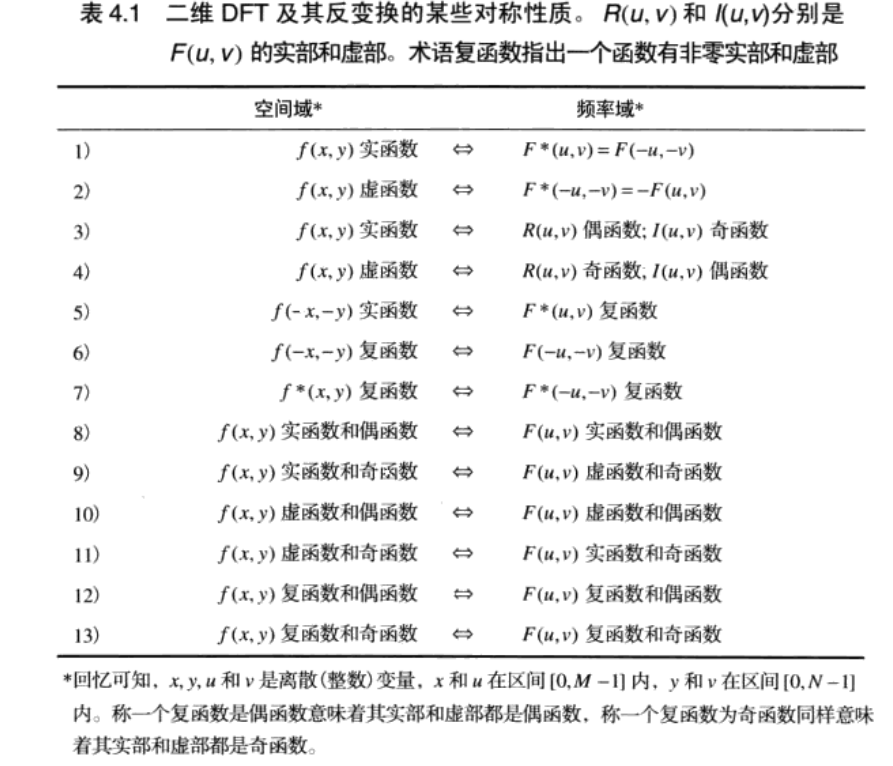
\includegraphics[width=0.8\textwidth]{symmetry_properties.png}
\caption{对称性质}
\label{fig:1}
\end{figure}

\subsubsection{Fourier Spectrum and Phase Angle 傅里叶谱和相角}

The $arctan$ must be computed using a four-quadrant arctangent.

$arctan$必须使用四象限反正切来计算。

The Fourier transform of a real function is conjugate symmetric,which imply that the spectrum has even symmetry about the origin:

实函数的傅里叶变换是共轭对称的,表明谱是关于原点偶对称的:

\begin{equation} \label{4.38}
|F(u,v)|=|F(-u,-v)|
\end{equation} 

The pahse angle exhibits the following odd symmetry about the origin:

相角关于原点奇对称:

\begin{equation} \label{4.39}
\phi(u,v)=-\phi(-u,-v)
\end{equation} 

\begin{equation} \label{4.40}
F(0,0)=\sum_{x=0}^{M-1}\sum_{y=0}^{N-1}f(x,y)
\end{equation} 

The zere-frequency term is proportional to the average value of $f(x,y)$.

即零频率项与$f(x,y)$的平均值成正比。

\begin{equation} \label{4.41}
F(0,0)=MN\frac{1}{MN}\sum_{x=0}^{M-1}\sum_{y=0}^{N-1}=MN\overline{f}(x,y)
\end{equation} 

$\overline{f}$ denotes the average value of $f$.

$\overline{f}$表示$f$的平均值。

The components of the spectrum of the DFT determine the amplitude of the sinusoids that combine to form the resulting image.,In DFT a large amplitude implies a greater prominence of a sinusoid of that frequency in the image.

DFT的谱的分量决定正弦波的幅度,这些正弦波结合起来可形成结果图像。图像的DFT变换中,较大的幅度意味着图像中该频率的正弦波比较突出。

The phase is a measure of displacement of the various sinusoids with respect to their origin.

相位是各个正弦分量关于原点的位移的度量。

While the magnitude of the 2-D DFT is an array whose components determine the intensities in the image,the corresponding phase is an array of angles that carry much of the information about where discernable objects are located in the image(and determine shape characteristics and feature content).

当二维DFT的幅度是一个阵列时,其分量决定了图像中的灰度,相应的相位则是一个角度的阵列,它携带较多关于图像中可辨别的物体定位的信息(还有决定形状特点和特性内容)。 

\subsubsection{The 2-D Convolution Theorem 二维卷积定理}

\begin{equation} \label{4.42}
f(x,y)\star h(x,y)=\sum_{m=0}^{M-1}\sum_{n=0}^{N-1}f(m,n)h(x-m,y-n)
\end{equation} 

$x=0,1,2,\ldots,M-1$ and $y=0,1,2,\ldots,N-1$

To obtain the same convolution result between the "straight" representation of the convolution equation approach and the DFT approach,functions in the latter must be padded prior to computing their transforms.

若要使``直接'' 卷积公式法与DFT方法产生的卷积结果相同,后者必须对函数补足周期再计算它们的变换。

Let $f(x,y)$ and $h(x,y)$ be two image arrays of sizes $A\times B$ and $C\times D$ Avoid wraparound error($f(x,y)$ and $h(x,y)$):

令$f(x,y)$ 和 $h(x,y)$分别是大小为 $A\times B$ 和 $C\times D$像素的图像阵列,避免缠绕错误(二维下):

Append zeros to both functions so that they have the same length,denoted by P.

把0加到两个函数中,使它们具有相同的长度,用P表示。

\begin{equation} \label{4.43}
f_{p}(x,y) = \left\{ \begin{array}{ll}
f(x,y) & \textrm{$0\leq x\leq A-1$ and $0\leq y\leq B-1$}\\
0 & \textrm{$A\leq x\leq P$ or $B\leq y\leq Q$ }\\
\end{array} \right.
\end{equation}

\begin{equation} \label{4.44}
h_{p}(x,y) = \left\{ \begin{array}{ll}
h(x,y) & \textrm{$0\leq x\leq C-1$ and $0\leq y\leq D-1$}\\
0 & \textrm{$C\leq x\leq P$ or $D\leq y\leq Q$ }\\
\end{array} \right.
\end{equation}

with 

$P\geq A+C-1$ and $Q\geq B+D-1$

DFT algorithms tend to execute faster with arrays of even size,so select P and Q as the smallest even integers.

一般DFT算法对偶数尺寸阵列执行较快,因此P和Q最好选择最小偶整数。

\subsubsection{Summary of 2-D Discrete Fourier Transform Properties 二维离散傅里叶变换性质小结}

\newpage

\begin{figure}[!htb] %插图
\centering
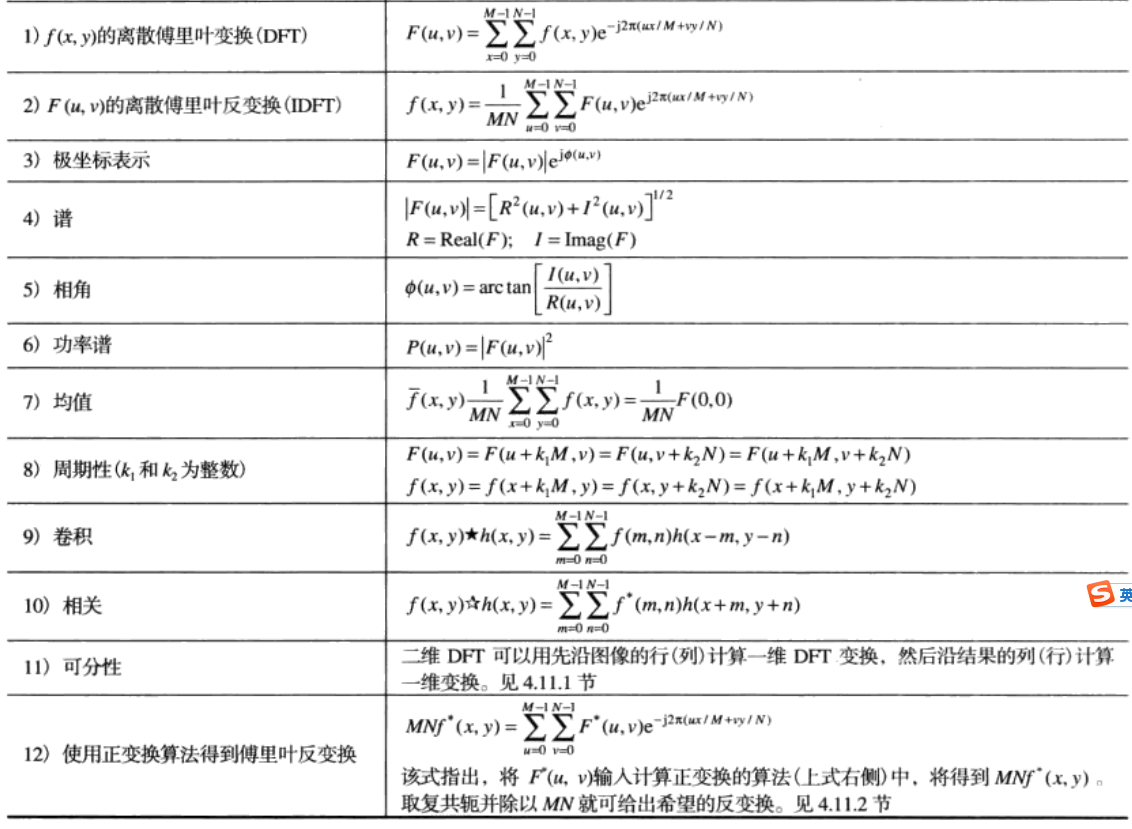
\includegraphics[width=1\textwidth]{DFTsummary.png}
\caption{DFT定义及相应表达式总结}
\label{fig:2}
\end{figure}\newpage

\begin{figure}[!htb] %插图
\centering
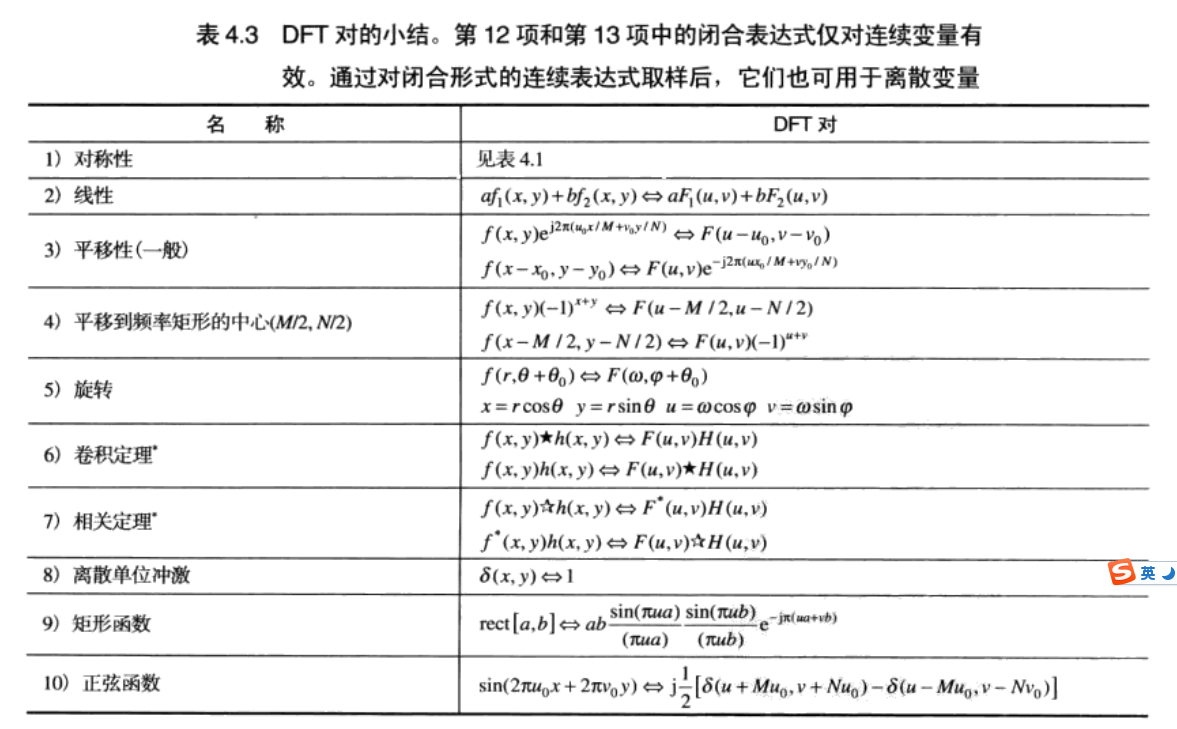
\includegraphics[width=1\textwidth]{summary_of_DFTpairs.png}
\caption{DFT对的小结}
\label{fig:3}
\end{figure}\newpage



\subsection{The Basic of Filtering in the Frequency Domain 频率域滤波基础}

Filtering techniques in the frequency domain are based on modifying the Fourier transform to achieve a specific objective and then computing the inverse DFT to get us back to the image domain.

频率中的滤波技术是以如下处理为基础的:修改傅里叶变换以达到特殊目的,然后计算IDFT返回到图像域。





%------------------------------------------------------------------------
\end{document}
